\chapter{Intégration dans l'équipe de projet}

\chapter{Montée en compétence}
Lorsque j'ai débuté mon stage je n'avais aucune visibilité sur le projet.
J'ai du me documenter et poser un tas de questions pour comprendre comment été structuré le projet d'une part et comment il fonctionné d'autre part. Ensuite il m'a fallu comprendre comment se déroulé le processus de développement dans Capgemini.
Cette phase de montée en compétence s'est déroulé tout au long du stage.

\section{Processus de développement Capgemini}
\subsection{Identification des versions}
\label{versionning}
Les versions sont marquées par des labels qui doivent permettre d'identifier de façon non équivoque toutes les évolutions successives des composants pour pouvoir retrouver et extraire de la base d'archives toute version livrée au client ou livrée pendant les phases d'intégration ou de la validation interne.
\\\\
On distingue deux types de versions :
\begin{description}
	\item[Version majeure] : c'est une version complète du logiciel, c'est à dire qu'elle contient l'ensemble des composants du système
	\item[Version mineure] : c'est une version paertielle du logiciel, c'est à dire qu'elle ne contient qu'un sous-ensebmel des composants du système, qui constitue un delta par rapport à la version précédente
	(qui peut être une version majeure ou mineure) ; c'est en général le résultat d'une correction ou d'une évolution mineure.
\end{description}
Les labels de version sont structurés de telle sorte que cette dépendance entre versions soit mise en évidence.
\\La composition d'un label de version est de la forme \textsc{GxxRyyCzz}.
\\Dans ce sigle on retrouve :
\begin{description}
	\item[Révision] : Une révision est attachée à un composant. \'A chaque fois qu'un utilisateur archive une nouvelle version d'un composant, l'outil de gestion de configuration crée une nouvelle révision de ce composant.
	\item[Version et labels] : Une version permet d'identifier un ensemble cohérent de composants d'une application. L'identifiant de version est sous contrôle complet de l'équipe de projet. Par exemple la première version est la G1R0C0, puis les suivantes seront les
	G1R1C0 puis la G2R0C0.
	\item[Tronc et branches] : Le \textit{tronc} supporte les versions principales. En cas de travaux parallèles sur plusieurs versions (par exemple la correction d'une anomalie sur une version n-1 et développement de la version n), on crée une branche qui va permettre de modifier une version déjà livrée.
	\\
\end{description}
\textbf{Exemple} : La branche G1R0 contient les versions correctives G1R0C1 et G1R0C2 qui intégrent des correctifs d'anomalies idnetifiées sur la version G1R0C0 préalablement livrée.
\setlength{\unitlength}{1.3cm}

\begin{picture}(5,5)
	%texte
	\put(-2,4.4){Tronc}
	\put(-2,2.4){Branche G1R0}
	%traits haut
	\put(2.5,4.4){\vector(1,0){1.5}}
	\put(6.5,4.4){\vector(1,0){1.5}}
	\put(10.5,4.4){\vector(1,0){1.5}}
	%oblique
	\put(1.5,4){\vector(0.3,-1){0.5}}
	%traits bas
	\put(4.5,2.4){\vector(1,0){1.5}}


	\put(0,4){\framebox(2.5,0.8)[c]{G1R0C0}}
	\put(4,4){\framebox(2.5,0.8)[c]{G1R1C0}}
	\put(8,4){\framebox(2.5,0.8)[c]{G2R0C0}}

	\put(2,2){\framebox(2.5,0.8)[c]{G1R0C1}}
	\put(6,2){\framebox(2.5,0.8)[c]{G1R0C2}}
\end{picture}
\begin{colbox}{{HTML}{C7FF99}}{}
Durant mon stage j'ai participé à l'intégration de la 6ème version (G1R6C0) et au développement et à l'intégration de la 7ème version (G1R7C0).
\end{colbox}

\newpage

\subsection{Organisation des environnements de travail}

Le \textbf{référenciel} (\textit{Repository}) contient l'ensemble des révisions de chaque composant ainsi que les liens entre composants permettant d'identifier les versions successives de chaque application.
\\\\
Les \textbf{espaces de travail} (\textit{Workspaces}) sont les espaces utilisés pour développer, intégrer, valider et livrer chaque application.
\\
\begin{picture}(0,1)
	%Referenciel
	\put(0,-2){Référenciel}
	\put(0.7,-1.5){\oval(2,2)[t]}
	\put(-0.3,-2.5){\line(0,1){1}}
	\put(1.7,-2.5){\line(0,1){1}}
	\put(0.7,-2.5){\oval(2,2)[b]}
	%fleches
	\put(1.7,-1.5){\vector(1,0){6}}
	\put(2.6,-1.4){Extraction des composants}

	\put(7.7,-2.5){\vector(-1,0){6}}
	\put(2.6,-2.4){Archivage des composants}
	%espaces de travail x+8
	\put(7.8,-2){Espaces de travail}
	\put(8.2,-2.6){Composants}
	\put(8.7,-1.5){\oval(2,2)[t]}
	\put(7.7,-2.5){\line(0,1){1}}
	\put(9.7,-2.5){\line(0,1){1}}
	\put(8.7,-2.5){\oval(2,2)[b]}
	%+0.3
	\put(9,-1.5){\oval(2,2)[t]}
	\put(8,-2.5){\line(0,1){1}}
	\put(10,-2.5){\line(0,1){1}}
	\put(9,-2.5){\oval(2,2)[b]}

	\put(9.3,-1.5){\oval(2,2)[t]}
	\put(8.3,-2.5){\line(0,1){1}}
	\put(10.3,-2.5){\line(0,1){1}}
	\put(9.3,-2.5){\oval(2,2)[b]}

\end{picture}
\\[6cm]
Quand l'activité le justifie, il est possible de devoir travailler simultanément sur plusieurs versions, en général :
\begin{itemize}
	\item Une version en \textbf{développement}
	\item Une version en \textbf{maintenance}\\
\end{itemize}
Il faut donc prévoir autant d'espaces de travail disponibles et ceci pour les différentes phases du cycle de développement :
\begin{itemize}
	\item Développement et tests unitaires
	\item Intégration et validation
	\item Livraison (effectuée sur la palte-forme de qualification)
\end{itemize}

\section{Cycle de développement}

Le développement se déroule en cycle en V :
%\begin{description}
  %\item[Spécifications] Le prestataire et le client communique pour valider les spécifications de la version.
  %\item[Chiffrage] Le prestataire fait un chiffrage et convient notamment des délais de livraison.
  %\item[Répartition des tâches] Le chef de projet répartie les tâches en fonction des domaines de compétence et de manière équilibré entre les développeurs.
  %\item[Développement] Les développeurs réalise les tâche demandées en suivant les spécifications.
  %\item[]



\section{Architecture du projet}
\subsection{Architecture technique}
L'architecture technique repose sur des machines virtuelles (excepté la BDD).
Voici une liste des infreastructures présentes :
\begin{description}
	\item[Serveur WAS] C'est le serveur qui délivre l'application à l'utilisateur. En effet, il s'y connecte via le GASSI du client avec le protocole HTTP ou via un VPN avec le protocole SSL. Il fonctionne sur une machine Linux avec le serveur d'application JOnAS\footnote{Java Open Application Server}.
\item[Serveur ArcGIS] Il traite les données SIG via le serveur ArcGIS délivré par l'éditeur Esri. Il fait le pont entre le serveur de base de données et le serveur WAS et accède aussi, via une architecture REST et SOAP à des interfaces Externes pour diverses missions. Par exemple avec l'application \textit{SIGEO}, développé par Capgemini pour récupérer les \textit{tuiles} de fond de plan.
\item[Serveur d'impression] En raison de la charge induite par la génération des PDF destiné à l'impression de fond de plan (certains au format A0), des serveurs sont dédiés à cette tâche. Il fonctionne avec le serveur ArcGIS.
\item[Serveur de base de données] Le serveur de base de données est PostGreSQL et permet de gérer l'accès et le stockage des données.\\
\end{description}

\'Etant donné la charge sur l'application (rappel : 1150 utilisateur simultanés par jour) il existe plusieurs instances de serveurs et la communication d'un serveur à un autre se fait via des répartiteurs de charges qui vont requêter le bon serveur au bon moment afin d'équilibrer la charge de travail entre les différents serveurs. De ce fait il y a, en plateforme de production :

\begin{itemize}
	\item 3 Serveurs WAS
	\item 8 Serveurs ArcGIS pour la France Métropolitaine et 2 pour les DOM
	\item 1 Serveur de base de données
	\item 4 Serveurs d'impressions\\
\end{itemize}
Pour une meilleure visibilité, vous pourrez trouvez le shéma d'achitecture technique en annexe \ref{archtech}.

\subsection{Architecture logicielle}

Geofibre est composé de 4 briques logiciel :
\begin{description}
	\item[gfi-bdd] Ce projet est lié à la structure des données du projet et contient les différents scripts PostgreSQL, fonctions et vues du projet. Ainsi que les différentes données liées à la configuration.
	\item[gfi-expl] Ce projet est liés à l'exploitation des serveurs faisant tourner le projet. Il contient majoritairement des scripts liés à la configuration des serveurs, des droits d'utilisation.
	\item[gfi-front] Ce projet est lié à l'IHM de l'application. Il contient du code en langage ActionScript 3 compilé par Adobe Flex.
	\item[gfi-back] Ce projet est lié au backoffice de l'application. Il contient du code Java tournant sur un serveur afin de requêter en REST et SOAP le serveur ArcGIS.
\end{description}
\begin{figure}[h]
	\captionbox{Arborescence du projet Geofibre\label{fig:dummy}}{
	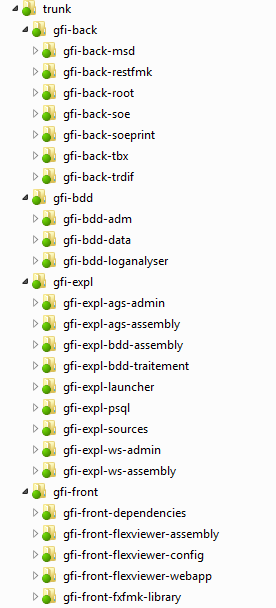
\includegraphics[width=7cm]{images/arborescence.png}
	}
\end{figure}
\chapter{Version G1R6C0}
Je suis arrivbé en cours de dev
\section{Spécifications}
\section{Développement}
\section{Rédaction des tests unitaires}
\section{Qualité de code}
\section{Intégration}
vague d'intégrationjusqu'il n'y a plus d'ano critiques
\subsection{Tests d'intégration des DOM}
\subsection{Tests de non-régression de la France Métropolitaine}
\subsection{Correction d'anomalies}

\chapter{Maintenance}
Pendant la phase de spécifications de la G1R7
\section{Correction d'anomalies éligibles à la G1R7}


\chapter{Version G1R7C0}
Cette version est essentiellement  fonctionnelle et dédiée à la prise en compte des paliers RIP et DSP.
Détail des items embarqués :
\begin{itemize}
\item Migration des RIP LTHD et CAPS de TIGRE
\item Configuration d’un ensemble de RIP
\item Gestion de valeurs par défaut sur l’IHM pour faciliter les actions de création/modification
\item Prise en compte des impacts sur les interfaces avec IPON (dont flux supplémentaires)
\item Prise en compte des impacts sur la Publication du SD.
\item Prise en compte des impacts sur la symbologie des immeubles
\item Ajout de filtrages RIP/Orange
\item Mise en conformité des études RIP existantes dans Geofibre
\item	Enveloppe MCO de la DS PIAR
\item Modification de la définition des diamètres des câbles pour l'extraction de l'annexe C3a (avec table de correspondance).
\item Evolution réglementaire de l’Annexe D8 (exports OPGC afin de différencier le mode de pose (Aérien ou Souterrain) et de visualiser le nombre de câbles sur les parcours (dont information de mode de pose liée au parcours).
\item Changement d’identification sur les nouveaux appuis ERDF (Exxxxxx au lieu de ERDFxxx), sans rattrapage de l’existant.
\item Des utilisateurs spécialisés sur l’activité RIP vont être ajoutés sur l’IHM GeoFibre.
\end{itemize}
D’un point de vue technique, la seule évolution concerne les flux IPON->GFI : IPON enverra un fichier Orange et un fichier RIP pour les câbles et les points techniques.
Aucune autre incidence sur l’architecture : le nombre des  nouveaux utilisateurs n’est pas de nature à saturer les ressources serveurs.

\section{Spécifications}
\section{Développement}
\subsection{Exemple}
\section{Rework}
\subsection{Exemple}
\section{Intégration}
